\subsection{UCW7 - Visualizza Classifica}
\begin{figure}[!h]
\centering
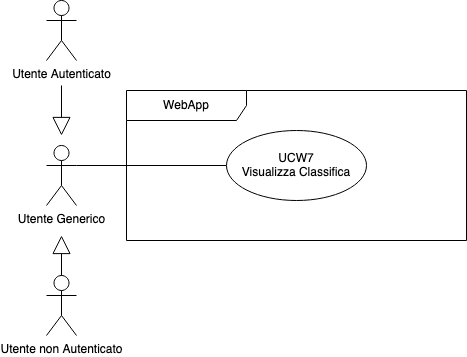
\includegraphics[scale=0.5]{UC_images/UCW7.png}
\caption{UCW7 - Visualizza Classifica}
\end{figure}
\begin{center}
\end{center}
\begin{itemize}
	\item \textbf{Descrizione}: L'utente generico visualizza la classifica dei locali presenti sulla piattaforma Sweeat.
    \item \textbf{Attore primario}: Utente generico.
    \item \textbf{Precondizione}: L’utente si trova all’interno della piattaforma Sweeat.
    \item \textbf{Postcondizione}: L’utente visualizza a schermo la classifica dei migliori locali gastronomici prodotta dal sistema senza alcun filtro applicato e con i parametri di ordinamento di default.
    \item \textbf{Scenario principale}: 
    \begin{enumerate}
        \item Un utente generico accede al sistema;
        \item L’utente seleziona la funzionalità visualizza classifica.
    \end{enumerate}
    \item \textbf{Sottocasi}:
    \begin{enumerate}
        \item Visualizza nomi locali (UCW7.1 §3.8.1);
        \item Visualizza punteggi totali (UCW7.2 §3.8.2);
        \item Visualizza categorie (UCW7.3 §3.8.3);
        \item Visualizza foto (UCW7.4 §3.8.4).
    \end{enumerate}
\end{itemize}

\begin{figure}[H]
    \centering
        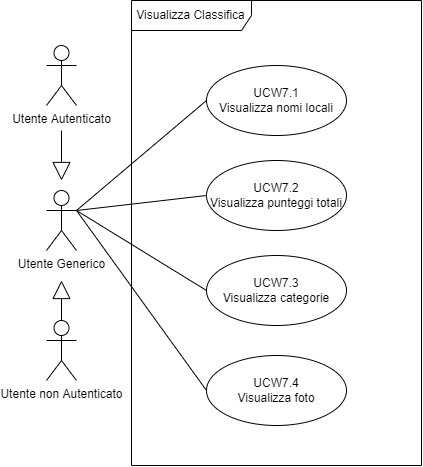
\includegraphics[scale=0.5]{UC_images/UCW7-1.png}
        \caption{Sottocasi UCW7}
\end{figure}

\subsubsection{UCW7.1 - Visualizza nomi locali}
\begin{itemize}
	\item \textbf{Descrizione}: L'utente generico visualizza i nomi dei locali presenti nella classifica.
    \item \textbf{Attore primario}: Utente generico.
    \item \textbf{Precondizione}: L’utente si trova all’interno della piattaforma Sweeat.
    \item \textbf{Postcondizione}: L’utente visualizza la lista dei nomi dei locali presenti nella classifica.
    \item \textbf{Scenario principale}: 
    \begin{enumerate}
        \item Un utente generico accede al sistema;
        \item L’utente seleziona la funzionalità visualizza classifica.
    \end{enumerate}
\end{itemize}

\subsubsection{UCW7.2 - Visualizza punteggi totali}
\begin{itemize}
	\item \textbf{Descrizione}: L'utente generico visualizza i punteggi totali dei locali presenti nella classifica. I punteggi totali sono ottenuti tenendo conto dei punteggi relativi a foto, testi ed emoji.
    \item \textbf{Attore primario}: Utente generico.
    \item \textbf{Precondizione}: L’utente si trova all’interno della piattaforma Sweeat.
    \item \textbf{Postcondizione}: L’utente visualizza i punteggi totali associati ai locali presenti nella classifica.
    \item \textbf{Scenario principale}: 
    \begin{enumerate}
        \item Un utente generico accede al sistema;
        \item L’utente seleziona la funzionalità visualizza classifica.
    \end{enumerate}
\end{itemize}

\subsubsection{UCW7.3 - Visualizza categorie}
\begin{itemize}
	\item \textbf{Descrizione}: L'utente generico visualizza le categorie a cui appartengono i locali presenti nella classifica.
    \item \textbf{Attore primario}: Utente generico.
    \item \textbf{Precondizione}: L’utente si trova all’interno della piattaforma Sweeat.
    \item \textbf{Postcondizione}: L’utente visualizza le categorie associate ai locali presenti nella classifica.
    \item \textbf{Scenario principale}: 
    \begin{enumerate}
        \item Un utente generico accede al sistema;
        \item L’utente seleziona la funzionalità visualizza classifica.
    \end{enumerate}
\end{itemize}

\subsubsection{UCW7.4 - Visualizza foto}
\begin{itemize}
	\item \textbf{Descrizione}: L'utente generico visualizza le foto dei locali presenti nella classifica.
    \item \textbf{Attore primario}: Utente generico.
    \item \textbf{Precondizione}: L’utente si trova all’interno della piattaforma Sweeat.
    \item \textbf{Postcondizione}: L’utente visualizza le foto associate ai locali presenti nella classifica.
    \item \textbf{Scenario principale}: 
    \begin{enumerate}
        \item Un utente generico accede al sistema;
        \item L’utente seleziona la funzionalità visualizza classifica.
    \end{enumerate}
\end{itemize}

